\documentclass[conference]{IEEEtran}
\usepackage[spanish]{babel}
\usepackage[utf8]{inputenc}
\usepackage{blindtext, graphicx}
\usepackage{subfigure}
\usepackage{mdwmath}
\usepackage{mdwtab}
\usepackage{subfig}
\usepackage{amsmath}
\usepackage{array}
\usepackage{multirow}
\bibliography{myBibliography}

\begin{document}
\title{  Clasificación de canciones por género musical utilizando una red neuroral artificial y la API de Spotify }
\author{\IEEEauthorblockN{Moreno Vázquez Pedro Abraham}
\IEEEauthorblockA{Departamento de Estudios Multidisciplinarios\\ Divisi\'on de ingenier\'ias\\
Campus Irapuato-Salamanca\\
Yuriria, Guanajuato\\
Correo: pa.morenovazquez@ugto.mx}

\and
\IEEEauthorblockN{Moreno Ramírez Walter Alejandro }
\IEEEauthorblockA{Departamento de Estudios Multidisciplinarios\\ Divisi\'on de ingenier\'ias\\
Campus Irapuato-Salamanca\\
Yuriria, Guanajuato\\
Correo: wa.morenoramirez@ugto.mx}}

\maketitle
\renewcommand\abstractname{Abstract}
\begin{abstract}
Here we go. \\
\end{abstract}



\begin{IEEEkeywords}
Red nueronal artificial.
\end{IEEEkeywords}

\tableofcontents

\IEEEpeerreviewmaketitle
\section{Introducción}
En búsqueda  de entender y replicar los sentidos que tenemos los seres humanos; su funcionamiento, procesamiento de la señal y el entendimiento de como nuestro cuerpo humano percibe e interpreta el mundo exterior, la ciencia se ha encargado de replicar y, en algunos casos, mejorar los sentidos que poseemos o de recuperar sentidos como el oido o el tacto en miembros humanos inutilisables o perdidos. Pero todo va aún más allá, existen ciencias encargadas de estudiar como se genera el conocimiento, la conciencia y como es el proceso dentro de nuestro cerebro cuando se esta realizando una acción tan cotidiana como es el escribir, hablar o un proceso aún más complejo como lo es el aprender. "Todos los procesos del cuerpo humano se relacionan en alguna u otra forma con actividad de neuronas. Las neuronas son un componente relativamente simple del ser humano, pero cuando millones de ellas se conectan en forma conjunta se hacen muy poderosas. \\
Lo que básicamente ocurre en una neurona biológica es lo siguiente: la neurona es estimulada o excitada a través de sus entradas (inputs) y cuando se alcanza un cierto umbral, la neurona se dispara o activa, pasando una señal hacia el axon. Así, el secreto de la "inteligencia", se sitúa dentro de estas neuronas interconectadas y de su interacción.\\

Por lo tanto, las Redes Neuronales biológicas:

\begin{itemize}
	\item Consisten en unidades de procesamiento que intercambian datos o información.
	\item Se utilizan para reconocer patrones, incluyendo imágenes, manuscritos y secuencias de tiempo.
	\item Tienen capacidad de aprender y mejorar su funcionamiento." \cite{walter}
\end{itemize}

\subsection{Redes Neuronales Artificiales}
Con las investigaciones realizadas por Alan Turing, en 1936, se dieron las primeras bases para estudiar el cerebro como una nueva forma de ver el mundo de la computación. Sin embargo, los fundamentos de la computación neuronal fueron creadas por dos científicos teóricos, el neurofisiólogo Warren McCulloch y el Matemático Walter Pitts, quienes en 1943 publicaron una teoría cerca de la forma de trabajar de las neuronas. Logrando modelar una red neuronal simple mediante circuitos eléctricos.\\
Como complemento, en 1949, Donald Hebb fue el primero en explicar los procesos del aprendizaje desde un punto de vista psicológico.\\
Y, en 1957, Frank Rosenblatt comenzó el desarrollo del Perceptron. Este tipo de red, es la más antigua y, aunque en sus inicios tenía muchas limitaciones; actualmente sus usos son variados entre los cuales se encuentran la identificación de patrones.\\

Una red neuronal artificial puede definirse como un conjunto de "redes interconectadas masivamente en paralelo de elementos simples y con organización jerárquica, las cuales intentan interactuar con los objetos del mundo real del mismo modo que lo hace el sistema nervioso biológico." \cite{walter} \\
Las redes neuronales artificiales presentan un gran número de características semejantes a las del cerebro. Pueden aprender de la experiencia, de generalizar de casos anteriores a nuevos casos, de abstraer características esenciales a partir de entradas que representan información irrelevante, etc. Esto hace que ofrezcan numerosas ventajas y que este tipo de tecnología tenga tantas aplicaciones en múltiples áreas.\\

\subsection{API Web de Spotify}
La API (Application Programming Interface) web de Spotify permite a los desarrolladores utilizar su aplicación para obtener datos del catálogo de música de Spotify. Los resultados de las peticiones a los servidores de Spotify dan como resultado archivos en formato JSON que proporciona información como artistas, álbumes y pistas directamente desde el catálogo de Spotify. Dependiendo de la autorización del usuario, la API también puede proporcionar a los programadores acceso a datos relacionados con el usuario, es decir, listas de reproducción y músicas guardadas en la biblioteca del usuario.\\

\begin{figure}[ht]
    \centering
    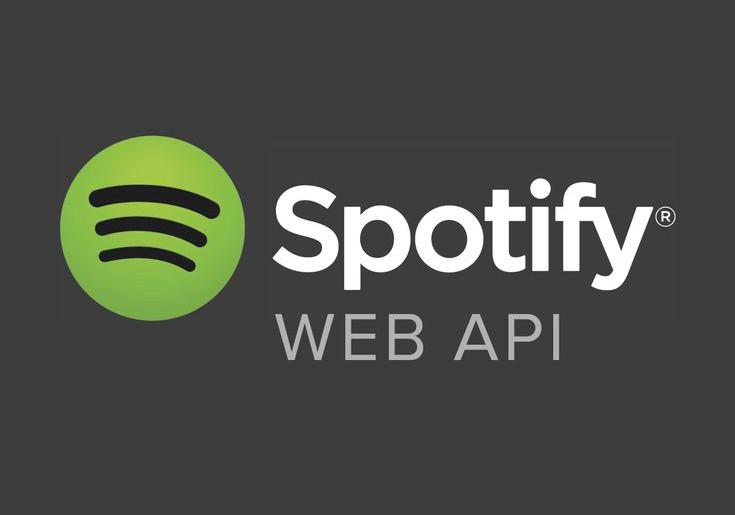
\includegraphics[scale=0.20]{./images/APIWebSpotify.jpg}
    \DeclareGraphicsExtensions.
    \caption{ Logo oficial de la API Web de Spotify. }
\end{figure}

Con la API web de Spositfy se pueden crear aplicaciones basando la lógica de negocio en el catálogo de música de Spotify. Estas aplicaciones son básicamente aplicaciones web integradas en el navegador basado en Chromium y bajo el sandbox que incluye Spotify. El desarrollo de una aplicación de Spotify es prácticamente idéntico que cualquier aplicación HTML5 que se crea hoy en día. Se puede combinar todo el conjunto de herramientas que se tienen a disposición como CSS, HTML y Javascript, así como cualquier framework Javascript como jQuery.

La API de Spotify permite, además de generar una estadística muy completa del uso de las canciones, obtener las características musicales de cada canción, ya sea de manera individual o en conjunto, mediante una playlist.\\
La características que se pueden obtener utilizando la API de Spotify son los siguientes: \\

\begin{itemize}
	\item \textbf{Danceability:} Una medida de 0.0 a 1.0 que tan buena es la canción para bailar.
	\item \textbf{Energy:} Una medida de 0.0 a 1.0 que indica el nivel de intensidad actividad.
	\item \textbf{Key:} La clave en que se encuentra la canción.
	\item \textbf{Loudness:} El volumén general en decibeles.
	\item \textbf{Mode:} Indica la modiladad de la canción.
	\item \textbf{Speechiness:} El nivel, de 0.0 a 1.0, de discurso en la canción.
	\item \textbf{Acousticness:} Una medida que indica que si la canción es acústica.
	\item \textbf{Instrumentalness:} Medidad que predice si la canción es instrumental o no.
	\item \textbf{Liveness:} Medida que indica la presencia de la audiencia en la grabación.
	\item \textbf{Valance:} Medida que indica el nivel de positividad en una canción.
	\item \textbf{Tempo:} El temp general de la canción en BPM.  \\
\end{itemize}

\subsection{Objetivo principal}
La finalidad de este trabajo es, mediante la utilización de una Red Neuronal Artificial (ANN), clasificar un conjunto de canciones en uno de cuatro géneros posibles: Metal, Mexicano, Pop y Rock. Utilizando la ANN para realizar las etapas de entrenamiento y pruebas. Comparando los resultados de la ANN con el algoritmo del vecino más cercano.\\

\section{Metodolog\'ia}
La conexión a los servidores de Spotify a través de su API, se realiza con scripts de Node.js, donde se realiza una autorización por parte del usuario para acceder a los datos. Para comenzar a realizar las peticiones se deben especificar dos claves que se generan para cada cuenta de desarrollador. Con estas claves un desarrollador se puede autenticar ante Spotify como usuario de su servicio, estas claves son: Client ID y Client Secret.\\

Para definir las clases prototipo se crearon 4 Playlist en Spotify, Pop 10, que hace referencia principalmente al pop de 2017, mexicano, que hace referencia a la música mexicana en general, Rock y Heavy Metal las cuales hacen referencia al género musical que se desea clasificar, la carátula de cada playlist se puede observar en la figura 2. A cada Playlist se agregó un total de 40 canciones, teniendo en total 160 canciones de muestras, de las cuales se obtuvieron las características musicales que Spotify provee. \\

\begin{figure}[htbp]
	\centering
	\subfigure{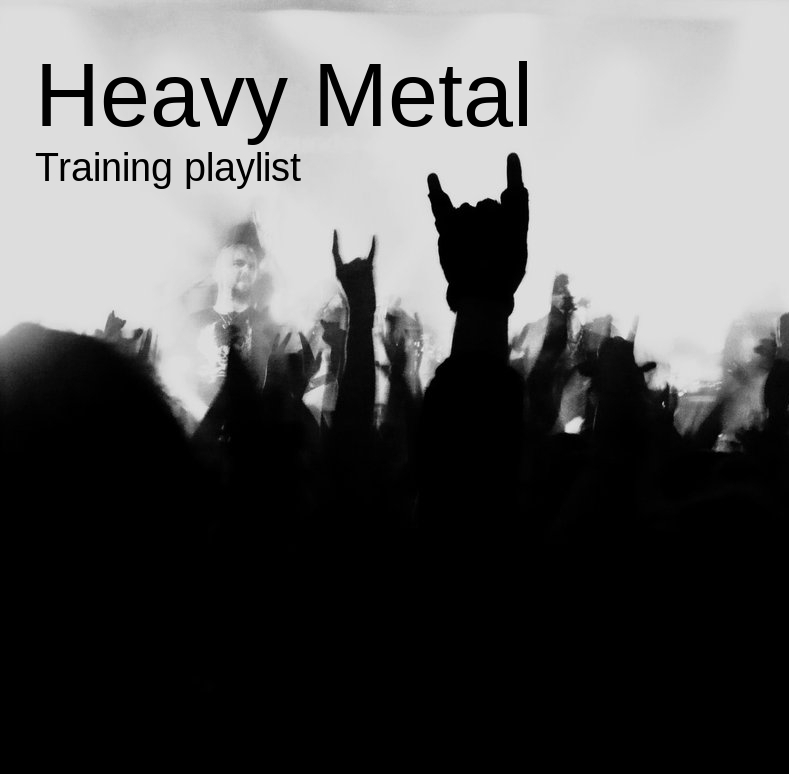
\includegraphics[scale=0.15]{./images/heavyMetalPlaylist.jpg}}
	\subfigure{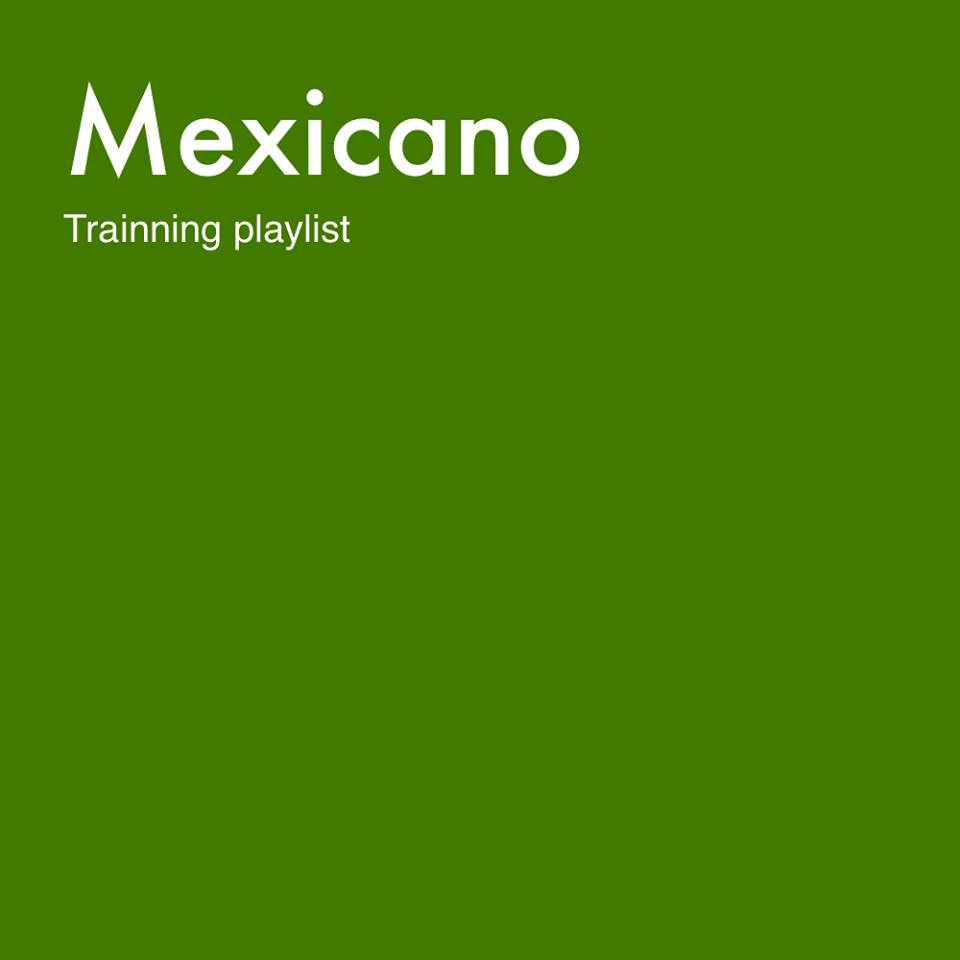
\includegraphics[scale=0.121]{./images/mexicanoPlaylist.jpg}}
	\subfigure{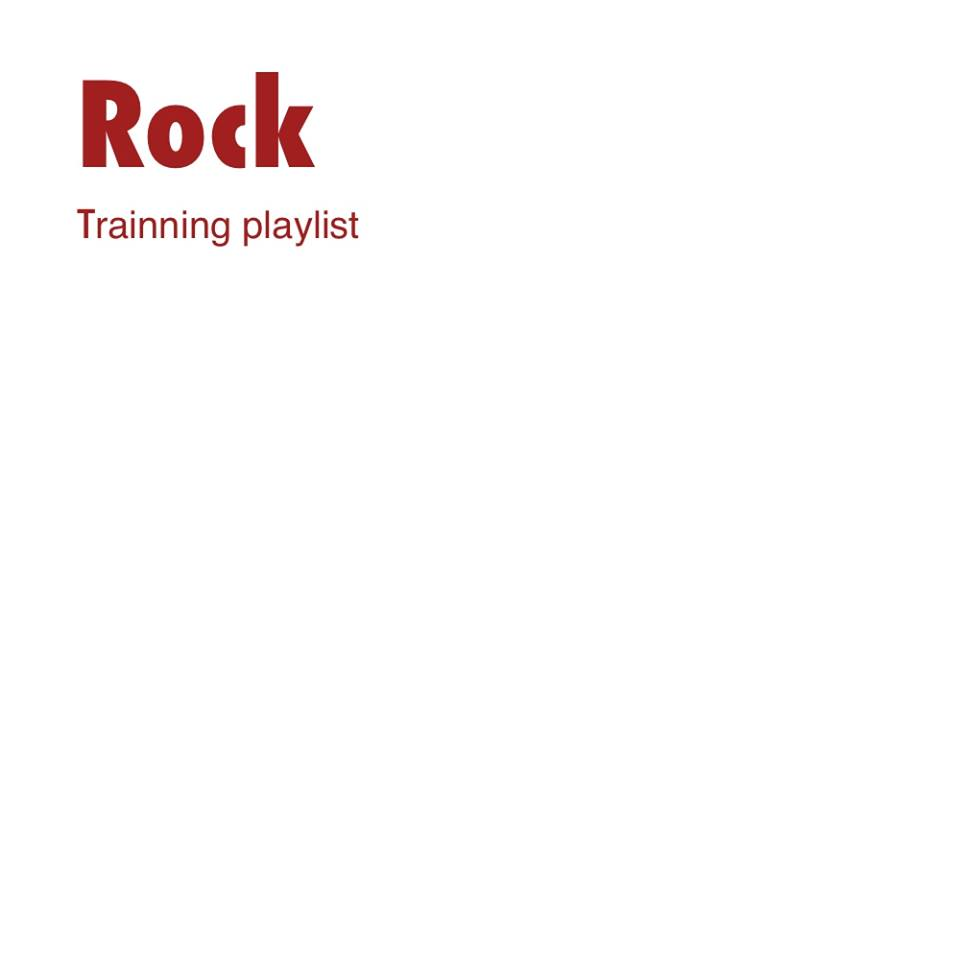
\includegraphics[scale=0.125]{./images/rockPlaylist.jpg}}
	\subfigure{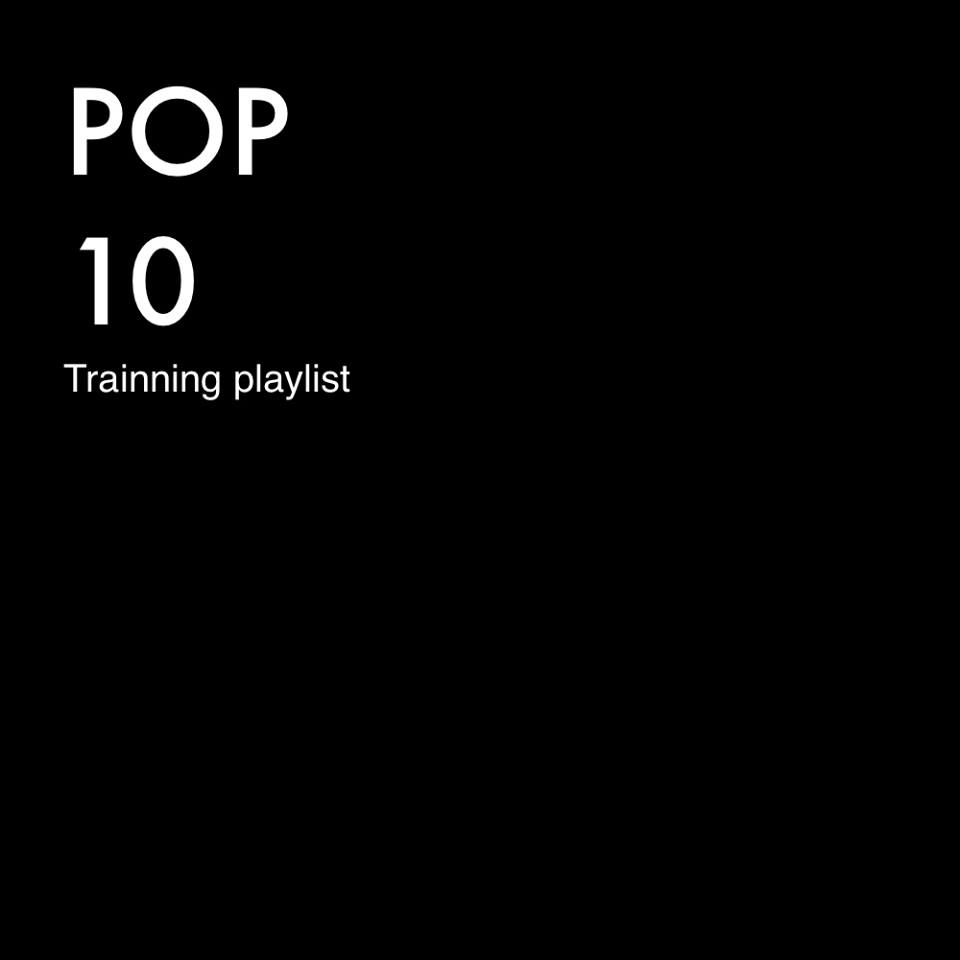
\includegraphics[scale=0.125]{./images/popPlaylist.jpg}}
	\caption{ Caratulas de las playlist creadas para ordenar las canciones que se utilizarán para entrenamiento y pruebas. }
\end{figure}

Para acceder a los datos Spotify genera un ID único para cada usuario, canción, playlist, etc., el cual sirve para hacer referencia a cada elemento dentro de los servidores de Spotify. Proporcionando las claves Client ID, Client Secret y el id de la playlist se pueden solicitar todos los id de cada canción en una playlist y con el conjunto de estas identificaciones las características, anteriormente mencionadas, de cada canción. Para realizar este procedimiento, se creó un script de Node.js, con el cual se obtienen las once características para cada canción de las 4 playlist.\\

\subsection{Etapa de entrenamiento}
Una ves obtenidas las características de cada canción, se adecuan al formato ARFF (Attribute-Relation File Format) de Weka, siendo este el archivo con el que se alimenta la Red Neuronal Artificial para la etapa de entrenamiento.\\
Dentro de la configuración de Weka, se selecciona, como método de clasificación, una Red Neuronal de un Perceptron Multicapa para realizar la etapa de entrenamiento.\\

Para probar la red neuronal Weka da la oportunidad de realizar una validación cruzada, por lo que se eleigíó que el software realizara una validación de este tipo con 10 iteraciones.\\

\begin{figure}[htbp]
	\centering
	\subfigure{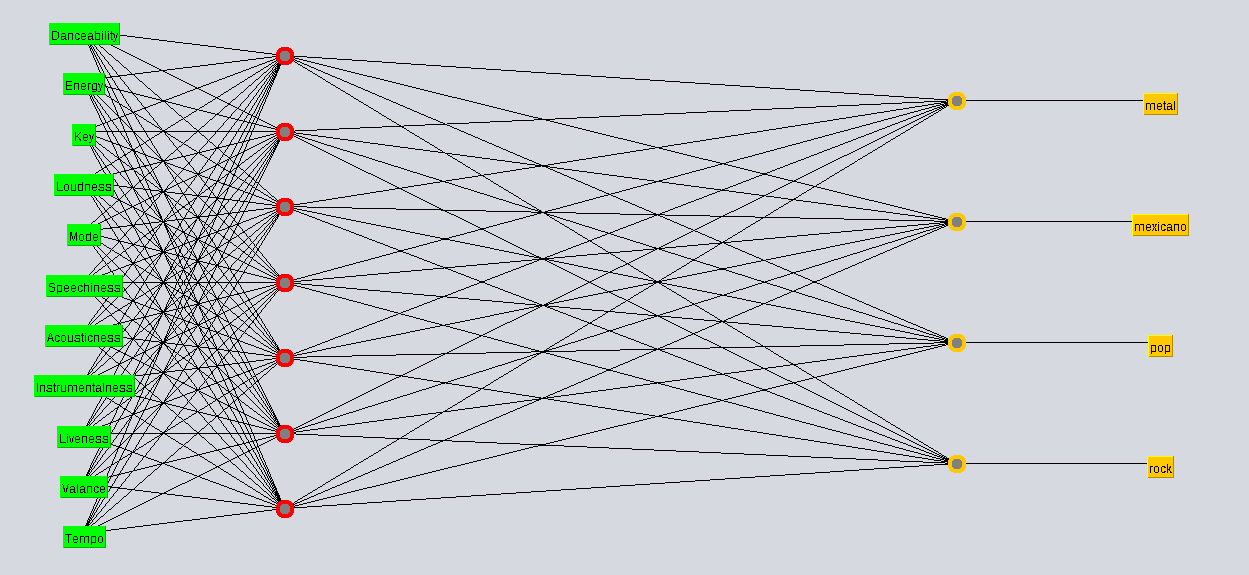
\includegraphics[scale=0.20]{./images/redNeuronal.png}}
	\caption{ Diagrama de la Red Neuronal de un Perceptron Multicapa generado por Weka. }
\end{figure}

El diagrama de la Red Neuronal de un Perceptron Multicapa que se creó con ayuda de Weka, mostrado en la Figura 3., muestra once Neuronas en la capa de entrada correspondientes a las once características para cada canción, siete en la capa oculta y cuatro para la capa de salida que corresponden a los cuatro generos en los que se desea clasificar las canciones.

\subsection{Vecino mas cercano}
Para comparar la exactitud de la red neuronal, se implementó el algoritmo del vecino m\'as cercano, utilizado en la etapa de pruebas de los métodos de clasificación supervizada. Este m\'etodo consiste en obtener la distancia euclidiana, ecuaci\'on (1), entre el elemento de prueba con cada una de las cuatro clases.

\begin{equation}
	D = \sqrt{ (C_n - S_{1} )^2 + (C_n - S_{2} )^2 + ... + (C_n - S_{11} )^2 }
\end{equation}

Donde:\\
\begin{itemize}
	\item $d$: es la distancia entre la canción de entrada y el prototipo de una de las 4 clases.
	\item $C_n$: es el prototipo para cada clase.
	\item $n = 1, 2, 3, 4$: indica el número de cada clase.
	\item $S_{1}, S_{2}, S_{3} ... S_{11}$: son las características de la canción de entrada. \\
\end{itemize}

La clasificación de cada nueva canción, utilizando este algoritmo, se hizó con la distancia menor de las tres distancias calculadas ya que es a la clase que más se acerca de acuerdo a sus características obtenidas con la API de Spotify.\\\\

\section{Resultados}

La red neuronal obtenida clasificó el 72.2 \% de las canciones en el generó correcto. Con la clasificación vista en la matriz de confusión de la tabla 1 se puede observar que la mayoría de los resultados de cada clase fueron verdaderos positivos, sin embargo la mejor clasificación se presento en el género pop y mexicano con una exactitud del 80.4\% y 92.1 \% respectivamente, demostrando que  ambos géneros son satisfactoriamente diferentes para que una canción futura se puda clasificar entre los dos géneros. Aunque el género Rock fue el que mas presento falsos positivos entre las diversas clases un caso especial se presentó entre este género y el metal, el 32.5 \% de falsos positivos de rock correspodian al metal, cosa que realmente no sorprende pues ambas, en algunos casos, usan los mismos instrumentos musicales, y por momentos llegan al mismo punto, ambos son rock solo que uno es mas ''pesado". 
 

\begin{table}[h]
	\renewcommand{\tablename}{Tabla}
	\centering
	\caption{Matriz de confusión}
	\label{my-label}
	\begin{tabular}{l|l|l|l|l|}
	\cline{2-5}
							& Mexicano  & Pop & Rock & Metal \\ \hline
	\multicolumn{1}{|l|}{Mexicano} & 35 & 2  & 3  & 0  \\ \hline
	\multicolumn{1}{|l|}{Pop} &  2  & 33  & 4  &  2 \\ \hline
	\multicolumn{1}{|l|}{Rock} &  2  &  6 &  19 & 13  \\ \hline
	\multicolumn{1}{|l|}{Metal} &  0  & 0  & 10  & 28  \\ \hline
	\end{tabular}
	\end{table}



\begin{table}[h]
\renewcommand{\arraystretch}{1.3}
\renewcommand{\tablename}{Tabla}
\caption{ Porcentaje de canciones clasificadas utilizando el algoritmo del vecino más cercano. }
\label{table_example}
\centering
\begin{tabular}{|c|c|c|}
\hline
CLASE (género) & Correctas & Incorrectas \\
\hline
Clase 1 (Metal) & 50.0 \% & 50.0 \% \\
\hline
Clase 2 (Mexicano) & 0.0 \% & 100.0 \% \\
\hline
Clase 3 (Pop) & 0.0 \% & 100.0 \% \\
\hline
Clase 4 (Rock) & 40.0 \% & 60.0 \% \\
\hline
Total & 22.50 \% & 77.50 \% \\
\hline
\end{tabular}
\end{table}

La tabla 2. muestra el resultado del algoritmo del vecino más cercano. La información que nos proporciona este tabla, indica el grado de exactitud con el que el algoritmo del vecino más cercano puede clasificar una nueva canción. \\

\section{Conclusiones}
La red neuronal artificial obtenida da suficiente exactitud para uso recreativo, lo que nos dice que las características usadas fueron las indicadas para hacer este tipo de clasificación. Cabe destacar que algunos elementos se les considera que no fue errónea su clasificación si no que la canción tambien puede pertenecer a ese genero y sería interesante explorar una clasificación con multiples salidas. 

\begin{thebibliography}{1}

\bibitem{walter}  
Matich, D. J. (2001). Redes Neuronales: Conceptos Básicos y Aplicaciones. Historia, 55. Retrieved from \\
\emph{$https://www.frro.utn.edu.ar/repositorio/catedras/quimica$
$/5 _ anio/orientadora1/monograias/matich-redesneuronales.pdf$}


\end{thebibliography}



\end{document}